\documentclass[a4paper,11pt]{article}

\usepackage[top=24mm,bottom=25mm,left=24mm,right=24mm]{geometry}
\usepackage{fontspec}
\usepackage{microtype}
\usepackage{amsmath,amssymb,bm}
\usepackage{booktabs}
\usepackage{array}
\usepackage{graphicx}
\usepackage{float}
\usepackage{tikz}
\usetikzlibrary{arrows.meta,positioning,shapes.geometric}
\usepackage{enumitem}
\usepackage{xcolor}
\usepackage{hyperref}
\usepackage{xurl}
\usepackage{xspace}

\hypersetup{
  colorlinks=true,
  linkcolor=blue!45!black,
  citecolor=blue!45!black,
  urlcolor=blue!55!black,
  pdftitle={A Portable GPU Implementation of Boltzmann Particle Hydrodynamics with Massively},
  pdfauthor={Akira Hayakawa}
}
\graphicspath{{../workspace/plot/}}
\setlength{\emergencystretch}{3em}
\setlist{nosep}

\newcommand{\bphgpu}{\texttt{bph-gpu}\xspace}
\newcommand{\massively}{\texttt{massively}\xspace}
\newcommand{\cubecl}{CubeCL\xspace}
\newcommand{\vect}[1]{\bm{#1}}
\newcolumntype{L}[1]{>{\raggedright\arraybackslash}p{#1}}

\title{A Portable GPU Implementation of\\
Boltzmann Particle Hydrodynamics with Massively}
\author{Akira Hayakawa}
\date{July 18, 2026}

\begin{document}
\maketitle

\begin{abstract}
Particle methods provide complementary routes to computational fluid dynamics.
Smoothed Particle Hydrodynamics (SPH) discretizes continuum equations through
kernel-weighted interactions among neighboring material particles, whereas
Boltzmann Particle Hydrodynamics (BPH) represents a velocity distribution with
Monte Carlo particles and alternates free flight with stochastic relaxation in
Cartesian cells.  BPH is attractive for high-Mach-number flow and vacuum, but
its sampling fluctuation demands large particle populations and therefore high
memory throughput.  This paper presents \bphgpu, a portable GPU implementation
in Rust built on \massively v0.80 and the \cubecl kernel language.  The central
implementation problem is that relaxation is local to cells whose particle
populations are irregular and change after every free-flight step, whereas the
updated state must remain aligned and be written per particle.  We resolve this
mismatch by composing sort-by-key, reduce-by-key, scatter, gather, masked
transform, and stream compaction.  These operations turn cell-local relaxation
into regular particle and cell arrays without a serial loop over cells or
contended atomic accumulation.  We derive the relaxation update, identify the
ordering and data-layout invariants required by the GPU realization, and give a
primitive-level algorithm detailed enough to reimplement it.  Operator checks
and a Sod shock tube calculation serve as a compact implementation
demonstration.  The focus is the GPU mapping rather than a new physical
validation of BPH or a benchmark claim about a particular device.
\end{abstract}

\begin{center}
\small
\textbf{Keywords:} Boltzmann Particle Hydrodynamics, Smoothed Particle
Hydrodynamics, GPU, Rust, parallel primitives, Monte Carlo particle method
\end{center}

\section{Introduction}

Particle methods have a long history in computational fluid dynamics.  SPH was
introduced independently by Lucy and by Gingold and Monaghan for astrophysical
gas dynamics \cite{lucy1977,gingold1977}.  It represents a continuum with
moving material particles and approximates fields and their gradients by
compact-support kernel sums over neighboring particles.  The resulting
Lagrangian, mesh-free description is particularly useful for large deformation,
moving interfaces, and free surfaces \cite{monaghan1992}.

A complementary line of development starts from kinetic theory.  Direct
Simulation Monte Carlo represents the molecular velocity distribution with
simulator particles and separates deterministic motion from stochastic
collisions \cite{bird1994}.  Isaka, Matsuda, and Boffin adapted this idea to
continuum gas flow as Molecular Hydrodynamics (MH), including internal degrees
of freedom, shocks, vacuum, and high-Mach-number states \cite{isaka2006}.
Murata et al. subsequently analyzed the stability and time-step behavior of the
continuum particle scheme \cite{murata2008}.  Later work published in the
proceedings of the Japan Society of Fluid Mechanics used the BPH designation
and investigated variable particle number and weight \cite{isaka2010}.  BPH,
as considered in this paper, follows the same stream--relax structure but
replaces explicit molecular collisions by a cell-local relaxation modeled
after the BGK approximation to the Boltzmann equation \cite{bgk}.

SPH and BPH are therefore related as Lagrangian particle approaches but are not
the same discretization.  SPH particles act as moving quadrature points for the
continuum equations and communicate through smoothing kernels.  BPH particles
sample a phase-space distribution; fixed cells localize relaxation, and density,
bulk velocity, and pressure are recovered as population moments.  Free flight
allows a BPH particle to traverse multiple cells in one update.  This supports
stable calculations beyond the usual explicit-grid CFL limit, although a large
time step still degrades accuracy through splitting error and numerical
viscosity \cite{isaka2006,murata2008}.

The particle representation is attractive for extreme states because density
is obtained from a nonnegative particle count and thermal energy from
nonnegative kinetic and internal energy.  Its principal cost is Monte Carlo
noise.  For a cell containing $N_g$ particles, ordinary sampling error scales
as $O(N_g^{-1/2})$; reducing it by a factor of ten requires approximately one
hundred times as many samples.  Memory capacity and throughput therefore become
central concerns.

GPU research on related particle methods establishes a useful computational
pattern.  GPU-accelerated SPH uses spatial cells, particle reordering, neighbor
processing, and on-device integration to handle millions of particles
\cite{crespo2011}.  All-device DSMC implementations likewise parallelize
particle motion, cell indexing, collisions, and sampling \cite{su2012}.  BPH
has the same broad opportunity for data parallelism, but its cell relaxation
requires segmented aggregation and redistribution rather than SPH kernel-force
evaluation or pairwise DSMC collision selection.

This work develops \bphgpu in Rust on top of \massively v0.80 and \cubecl
\cite{massively,cubecl}.  Its subject is the algorithmic mapping required to
execute BPH on a GPU.  The paper makes three contributions.  First, it states
the mathematical update that must be preserved by a parallel implementation,
including equal-mass and full-relaxation assumptions.  Second, it identifies
the GPU-specific obstacles: time-dependent cell membership, highly uneven cell
populations, transitions between particle and cell data, empty cells, and the
need to reorder every particle field consistently.  Third, it shows how the
public parallel primitives of \massively express each obstacle as a portable
composition over device-resident arrays.  A shock tube is included only to
demonstrate that the composed implementation executes the intended BPH cycle;
it is not presented as a comprehensive validation campaign.

\section{Theoretical Background}

\subsection{The BGK equation and operator splitting}

Let $\vect{x}$ be position, $\vect{c}$ molecular velocity, $\vect{F}$ external
acceleration, $n$ number density, and $f$ a normalized velocity distribution.
The BGK equation is
\begin{equation}
 \frac{\partial(nf)}{\partial t}
 + \vect{c}\cdot\nabla_{\vect{x}}(nf)
 + \vect{F}\cdot\nabla_{\vect{c}}(nf)
 = n\frac{f^{\mathrm{eq}}-f}{\tau},
 \label{eq:bgk}
\end{equation}
where $\tau$ is the relaxation time \cite{bgk}.  The equilibrium surrogate
$f^{\mathrm{eq}}$ used by BPH need not be Maxwellian.  It is sufficient for it
to be isotropic in velocity space and to preserve the mass, momentum, and total
energy moments,
\begin{equation}
 \int nf\,Q(\vect{c})\,d\vect{c}
 =\int nf^{\mathrm{eq}}\,Q(\vect{c})\,d\vect{c},
 \quad
 Q\in\left\{m,m\vect{c},\tfrac12m|\vect{c}|^2+e\right\}.
 \label{eq:moments}
\end{equation}
The implementation studied here uses a spherical-shell distribution for the
angular part of this equilibrium surrogate.

Equation~\eqref{eq:bgk} is split into transport and collision.  Conceptually,
one time step is
\begin{equation}
 \text{streaming: }(\vect{x},\vect{c})\longrightarrow
 (\vect{x}^{*},\vect{c}^{*}),
 \qquad
 \text{relaxation: }f^{*}\longrightarrow f^{n+1}.
\end{equation}
The numerical method repeats the order shown in Fig.~\ref{fig:loop}: compute
cell indices, reorder particles, relax, stream, and apply boundary conditions.
This ordering differs only in time labeling from a move--then--relax
description, because positions produced by one iteration are consumed by
relaxation in the next.  With no external force, the first-order streaming
update is
\begin{equation}
 \vect{x}^{n+1}=\vect{x}^{n}+\vect{c}^{n+1}\Delta t.
 \label{eq:stream}
\end{equation}
The numerical demonstrations in Section~4 use no external force.

\begin{figure}[H]
 \centering
 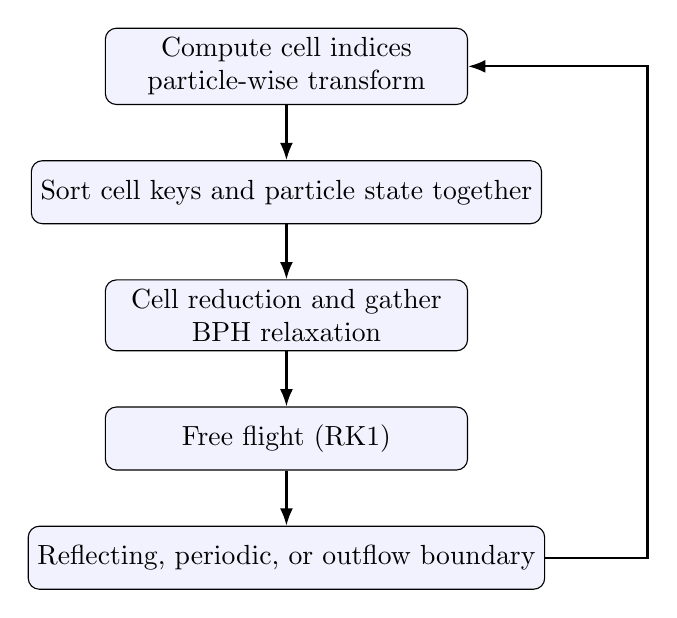
\begin{tikzpicture}[
   node distance=7mm,
   box/.style={draw,rounded corners,minimum width=46mm,minimum height=8mm,
               align=center,fill=blue!5},
   arr/.style={-{Latex[length=2.2mm]},thick}
 ]
  \node[box] (index) {Compute cell indices\\particle-wise transform};
  \node[box,below=of index] (sort) {Sort cell keys and particle state together};
  \node[box,below=of sort] (relax) {Cell reduction and gather\\BPH relaxation};
  \node[box,below=of relax] (move) {Free flight (RK1)};
  \node[box,below=of move] (bound) {Reflecting, periodic, or outflow boundary};
  \draw[arr] (index) -- (sort);
  \draw[arr] (sort) -- (relax);
  \draw[arr] (relax) -- (move);
  \draw[arr] (move) -- (bound);
  \draw[arr] (bound.east) -- ++(13mm,0) |- (index.east);
 \end{tikzpicture}
 \caption{One BPH time step.  In the GPU implementation, particle state remains
 resident on the device throughout the loop.}
 \label{fig:loop}
\end{figure}

\subsection{Particle state, heat-capacity ratio, and preconditions}

Particle $i$ has position $\vect{x}_i$, velocity
$\vect{c}_i=(u_i,v_i,w_i)$, mass $m_i$, internal energy $e_i$, and cell index
$g(i)$.  In addition to three translational degrees of freedom, a particle has
$s\geq0$ internal degrees of freedom.  The corresponding ratio of specific
heats is
\begin{equation}
 \gamma=1+\frac{2}{3+s}=\frac{s+5}{s+3}.
 \label{eq:gamma}
\end{equation}
Thus $s=0$ gives $\gamma=5/3$, while $s=2$ gives $\gamma=7/5$.

The formulation considered here assumes that particles participating in a
relaxation have equal masses and the same $s$.  The arithmetic mean in
Eq.~\eqref{eq:center} would have to be replaced by a mass-weighted mean for
variable particle masses.  The conservation derivation and numerical
demonstrations below therefore assume $m_i=m$.

\subsection{Relaxation within one cell}

Let $I_g$ be the set of particles in cell $g$ and $N_g=|I_g|$.  A cell with
$N_g<2$ cannot model a collision and is left unchanged.  For $N_g\geq2$, define
the mean and thermal velocities as
\begin{equation}
 \vect{U}_g=\frac{1}{N_g}\sum_{i\in I_g}\vect{c}_i,
 \qquad
 \vect{q}_i=\vect{c}_i-\vect{U}_g.
 \label{eq:center}
\end{equation}
The energy to be redistributed in the center-of-mass frame is
\begin{equation}
 E_g=\sum_{i\in I_g}
 \left(\frac12m|\vect{q}_i|^2+e_i\right).
 \label{eq:cellenergy}
\end{equation}
Equipartition assigns the post-relaxation translational kinetic and internal
energies in the ratio $3:s$,
\begin{equation}
 K_g^{\star}=\frac{3}{3+s}E_g,
 \qquad
 E_{\mathrm{int},g}^{\star}=\frac{s}{3+s}E_g.
 \label{eq:partition}
\end{equation}

For each particle, two independent uniform variates
$r_{1i},r_{2i}\in[0,1)$ produce
\begin{align}
 \mu_i &= 1-2r_{1i}, & \theta_i&=2\pi r_{2i},\\
 \vect{d}_i &=
 \left(\sqrt{1-\mu_i^2}\sin\theta_i,
       \sqrt{1-\mu_i^2}\cos\theta_i,\mu_i\right).
 \label{eq:shell}
\end{align}
Because $|\vect{d}_i|=1$, these vectors are uniformly distributed over the
unit sphere.  A finite sample does not have exactly zero vector sum, so it is
balanced within each cell:
\begin{equation}
 \widehat{\vect{d}}_i=\vect{d}_i-
 \frac{1}{N_g}\sum_{j\in I_g}\vect{d}_j,
 \qquad
 K_g^{\mathrm{raw}}=\sum_{i\in I_g}\frac12m
 |\widehat{\vect{d}}_i|^2.
 \label{eq:balance}
\end{equation}
The velocity scale is
\begin{equation}
 a_g=\sqrt{\frac{K_g^{\star}}{K_g^{\mathrm{raw}}}},
 \label{eq:scale}
\end{equation}
and the relaxed state becomes
\begin{equation}
 \vect{c}'_i=\vect{U}_g+a_g\widehat{\vect{d}}_i,
 \qquad
 e'_i=\frac{E_{\mathrm{int},g}^{\star}}{N_g}.
 \label{eq:update}
\end{equation}
The rescaling in Eq.~\eqref{eq:scale} requires
$K_g^{\mathrm{raw}}>0$.  With continuously sampled independent directions,
the degenerate event has probability zero for $N_g\geq2$, but a finite random
generator can still represent it.  The implementation guards the division and
sets the scale to zero; a reimplementation that requires conservation in this
exceptional case should resample the directions or supply a deterministic
zero-mean shell configuration.

\subsection{Conservation and numerical properties}

Equation~\eqref{eq:balance} gives
$\sum_i\widehat{\vect{d}}_i=\vect{0}$, and hence
\begin{equation}
 \sum_{i\in I_g}m\vect{c}'_i=mN_g\vect{U}_g
 =\sum_{i\in I_g}m\vect{c}_i.
\end{equation}
Cell momentum is therefore conserved.  The cross term also vanishes, giving
\begin{align}
 \sum_{i\in I_g}\left(\frac12m|\vect{c}'_i|^2+e'_i\right)
 &=\frac12mN_g|\vect{U}_g|^2+K_g^{\star}
   +E_{\mathrm{int},g}^{\star}\\
 &=\frac12mN_g|\vect{U}_g|^2+E_g.
\end{align}
Thus, for $K_g^{\mathrm{raw}}>0$ and exact arithmetic, total energy is conserved
as well.  Mass conservation is immediate for cell relaxation because it neither
creates nor removes particles.  An outflow boundary may, of course, reduce the
mass inside the computational domain.

A forward-Euler discretization of the BGK collision term permits a relaxation
probability $P=\Delta t/\tau$.  For viscous flow, relaxation can be sampled with
this probability to represent a finite mean free path.  Setting $P=1$ instead
produces the full-relaxation Euler model implemented by the current \bphgpu
code; a finite-$P$ Navier--Stokes viscosity model is not yet implemented.

The statement that BPH is not restricted by the CFL condition follows from
particles being able to cross cell boundaries.  It must not be interpreted as
saying that every time step is accurate.  Increasing $\Delta t$ increases
splitting error and numerical viscosity, and boundary processing must account
consistently for every crossing made during a long flight.

\section{GPU Mapping with Massively}

\subsection{Why cell relaxation is difficult on a GPU}

Free flight is particle-local, but relaxation is neither a purely particle-local
kernel nor a fixed-size cell stencil.  Every particle must first discover its
current cell.  The number of particles in a cell may range from zero to a large
fraction of the whole population, and the distribution changes at every step.
Assigning one thread or one fixed workgroup to each cell therefore creates both
load imbalance and an unknown local-storage requirement.  Conversely, assigning
one thread to each particle leaves the cell sums, means, and energy scale
unavailable without a many-to-one aggregation.

The implementation must consequently alternate between two index spaces.  The
particle space has length $N$ and is suitable for streaming, random sampling,
and final state updates.  The cell space has length $K$ and contains populations,
velocity sums, energies, and relaxation scales.  A practical GPU algorithm must
aggregate particle values into cells, represent empty cells, and redistribute
cell values to particles while preserving the association among all
structure-of-arrays columns.  Table~\ref{tab:challenges} summarizes how
\massively v0.80 supplies these transitions.

\begin{table}[H]
 \centering
 \footnotesize
 \caption{BPH GPU challenges and their realization with \massively v0.80.}
 \label{tab:challenges}
 \begin{tabular}{@{}L{42mm}L{46mm}L{48mm}@{}}
  \toprule
  BPH requirement & GPU difficulty & Massively composition \\
  \midrule
  Form current cell groups & membership changes after streaming &
  \texttt{sort\_by\_key} with one shared permutation \\
  Compute cell moments & uneven many-to-one aggregation &
  \texttt{reduce\_by\_key} on contiguous equal-key runs \\
  Include empty cells & reductions emit occupied keys only &
  zero-filled cell array followed by \texttt{scatter} \\
  Apply cell values to particles & results live in cell index space &
  key-indexed \texttt{gather} or an equivalent lazy indexed read \\
  Update only collidable cells & cells below two particles must be unchanged &
  masked \texttt{transform} or \texttt{gather\_where} \\
  Remove outflow particles & the particle population is dynamic &
  \texttt{remove\_where} with a boundary predicate \\
  \bottomrule
 \end{tabular}
\end{table}

\subsection{Execution model and data layout}

\bphgpu implements BPH in Rust using the \massively v0.80 parallel-algorithm library
and the \cubecl kernel language \cite{massively,cubecl}.  Particle data stay in
device memory throughout the time-stepping loop.  The runtime abstraction can
lower the same algorithm to WGPU, CUDA, or HIP; the numerical results reported
here use WGPU, while cross-backend equivalence and performance remain to be
measured.

Particle state is stored in separate contiguous arrays for
$x,y,z,u,v,w,e$, a structure-of-arrays (SoA) layout.  Any operation that
reorders particles computes one index permutation and applies it identically to
every state column, including mass if it is not a global constant.  Each
physical column therefore remains contiguous for coalesced particle-wise
access.  The particle arrays and the cell-key array must always have the same
length and particle ordering.

Cell arrays always have length $K$, including entries for empty cells.  A
reduction by key emits results only for nonempty cells, so the compact output
is scattered by cell index into a dense, zero-initialized array.  A gather then
distributes each cell value back to its member particles.  This
reduction--scatter--gather cycle is the bridge between cell-local physical
quantities and particle-level parallel work.

\subsection{Cell keys and ordering invariants}

Let $N$ be the number of particles and let a Cartesian grid contain
$K=n_xn_yn_z$ cells.  For cell widths $h_\alpha$ and lower domain coordinates
$x_{\alpha,\min}$, an interior particle receives
\begin{align}
 j_{\alpha i}&=\left\lfloor
 \frac{x_{\alpha i}-x_{\alpha,\min}}{h_\alpha}\right\rfloor,
 & 0\leq j_{\alpha i}<n_\alpha,\\
 g_i&=j_{xi}+n_x\left(j_{yi}+n_yj_{zi}\right),
 &0\leq g_i<K.
 \label{eq:cellkey}
\end{align}
Periodic or reflecting coordinates must be returned to the domain, and outflow
particles removed, before the next evaluation of Eq.~\eqref{eq:cellkey}.
Keys from the previous free-flight step must not be reused.

The key--state pairs are sorted in ascending $g_i$, applying the resulting
permutation to every particle field.  Stability among equal keys is not a
physical requirement; the required invariants are that equal keys form a
contiguous run and that all fields retain their particle association.  Spatial
sorting is also a standard building block in GPU SPH and DSMC implementations
\cite{crespo2011,su2012}.

\subsection{Massively primitive composition}

The names in Table~\ref{tab:challenges} correspond to the public algorithmic
interfaces of \massively v0.80: \texttt{sort\_by\_key},
\texttt{reduce\_by\_key}, \texttt{scatter}, \texttt{gather},
\texttt{lower\_bound}, \texttt{upper\_bound}, and masked transforms.  The
important point is their composition, not library-specific iterator or integer
conversion types.  The same decomposition can be reproduced in another GPU
framework that provides operations with equivalent semantics.

One way to make the ordering explicit is to sort the pairs $(g_i,i)$ by their
first component.  If $p$ is the resulting permutation, then
$g_{p_0}\leq g_{p_1}\leq\cdots\leq g_{p_{N-1}}$, and every particle field is
gathered in the order $p$.  Sorting key--state records directly is equivalent,
provided that all state fields receive exactly the same permutation.  The
ordering should be computed once per time step and shared by all fields.

The central reusable operation is a dense cell reduction.  Given sorted keys
$\vect{g}$ and particle values $\vect{a}$, reduction by key first returns
unique occupied keys $\vect{\kappa}$ and compact sums $\vect{s}$.  Scattering
them into a zero-initialized cell array gives
\begin{equation}
 (\vect{\kappa},\vect{s})=\operatorname{reduce\_by\_key}
 (\vect{g},\vect{a}),\qquad
 \vect{A}=\vect{0}_K,\qquad
 A_{\kappa_j}\leftarrow s_j.
 \label{eq:densereduce}
\end{equation}
This construction represents empty cells explicitly without a contended
particle-to-cell atomic accumulation.  The population of cell $g$ is the
difference between the upper and lower bounds of $g$ in the sorted key array.
Equivalently, it can be obtained by applying Eq.~\eqref{eq:densereduce} to a
particle array of ones.

For any dense cell field $A_g$, permutation by the particle keys constructs the
particle field $a_i=A_{g_i}$.  A GPU implementation may fuse this indexed read
with its consuming kernel or materialize the gathered particle array; both have
the same mathematical meaning.  Vector quantities such as $(u,v,w)$ may be
processed component-wise or as tuples, provided that the SoA fields remain
aligned.  A mask for $N_g\geq2$ selects particles eligible for relaxation, while
particles in smaller cells retain their previous state.

\subsection{Parallel relaxation}

The following sequence is sufficient to reimplement one full-relaxation BPH
collision step.  Here \textsc{DenseReduce} denotes
Eq.~\eqref{eq:densereduce}, \textsc{Gather}$(A,\vect{g})_i=A_{g_i}$, and all
particle maps are parallel.
\begin{enumerate}[label=\arabic*.]
 \item Compute $N_g$ and
       $\vect{S}_g=\textsc{DenseReduce}(\vect{g},\vect{c})_g$, then form
       $\vect{U}_g=\vect{S}_g/N_g$ for nonempty cells.
 \item Gather $\vect{U}_{g_i}$, save it until the end of relaxation, and center
       each velocity: $\vect{q}_i=\vect{c}_i-\vect{U}_{g_i}$.
 \item Compute
       $E_g=\textsc{DenseReduce}\bigl(\vect{g},
       \tfrac12m|\vect{q}|^2+e\bigr)_g$.
 \item Generate two independent uniform particle arrays and transform them by
       Eq.~\eqref{eq:shell} to obtain $\vect{d}_i$.
 \item Compute
       $\overline{\vect{d}}_g=
       \textsc{DenseReduce}(\vect{g},\vect{d})_g/N_g$ and set
       $\widehat{\vect{d}}_i=\vect{d}_i-
       \overline{\vect{d}}_{g_i}$.  This finite-sample correction, rather than
       isotropy only in expectation, is what enforces discrete momentum
       conservation.
 \item Compute
       $K_g^{\mathrm{raw}}=\textsc{DenseReduce}\bigl(\vect{g},
       \tfrac12m|\widehat{\vect{d}}|^2\bigr)_g$, followed by
       $K_g^\star$, $E_{\mathrm{int},g}^\star$, and $a_g$ from
       Eqs.~\eqref{eq:partition} and \eqref{eq:scale}.
 \item For cells with $N_g\geq2$, gather these cell values and write
       $\vect{c}'_i=\vect{U}_{g_i}+a_{g_i}\widehat{\vect{d}}_i$ and
       $e'_i=E_{\mathrm{int},g_i}^\star/N_{g_i}$.  Leave particles in cells
       with $N_g<2$ unchanged, and guard $K_g^{\mathrm{raw}}=0$ before the
       square root.
\end{enumerate}

After relaxation, Eq.~\eqref{eq:stream} advances positions and the selected
boundary operator is applied.  The next step then recomputes and sorts the cell
keys.  Independent random streams are required for the two angular variates;
changing the streams between time steps avoids repeating the same angular
sample.  A deterministic seed schedule is useful for repeatable tests, although
bitwise identity across backends is not assumed because random generators and
floating-point reduction order may differ.

\subsection{Memory traffic and performance considerations}

Particle parallelism avoids the load imbalance of assigning one thread to a
cell whose population may range from zero to many thousands.  It does not make
the algorithm free of global data movement.  Each time step performs several
full-particle passes, while sorting applies a permutation to every dynamic
particle column.  A comparison sort has $O(N\log N)$ work, and relaxation
requires multiple reductions and particle--cell mappings.  These stages are
therefore the principal candidates for profiling, but no timing attribution is
claimed without measurements of this implementation.

Fusing indexed reads with their consuming kernels can avoid some intermediate
arrays, but several stages still require temporary $N$- or $K$-element buffers.
Kernel fusion, persistent buffer reuse, a bounded-integer cell sort, and
sort-free aggregation are thus the principal optimization candidates.  The
asymptotic additional storage is $O(N+K)$.

\section{Implementation Demonstration}

The implementation is exercised at two levels.  Operator checks verify that
segmented reductions produce the prescribed dense cell sums, including zeros
for empty cells; one shared sort permutation keeps particle columns aligned;
subtracting and restoring the gathered cell velocity recovers the original
velocity; and the relaxation composition preserves the intended energy split
for nondegenerate shell samples.  These checks target the dataflow invariants
on which the GPU mapping depends.

A Sod shock tube \cite{sod1978} provides a compact end-to-end demonstration.
The unit interval is divided into $K=2{,}000$ cells with
$\Delta t=\Delta x=5\times10^{-4}$.  The initial left and right states have
density ratio $8:1$, pressure ratio $10:1$, and zero bulk velocity.  They are
represented by 4,000 and 500 equal-mass particles per cell, respectively, for
$N=4{,}500{,}000$ particles.  The calculation uses $s=2$
($\gamma=7/5$), full relaxation, single-precision state, the WGPU backend, and
advances to $t=0.15$.  Density is reported as the cell population divided by
the initial left-state population of 4,000.

\begin{figure}[H]
 \centering
 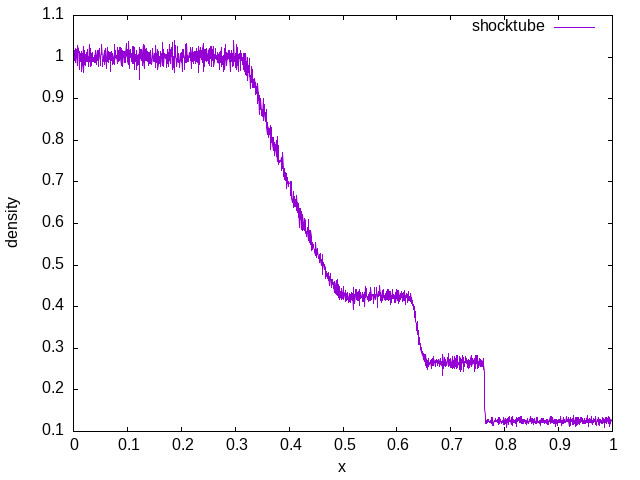
\includegraphics[width=0.78\linewidth]{shocktube.jpeg}
 \caption{Normalized cell density for the Sod shock tube computed by
 \bphgpu.  The rarefaction, contact discontinuity, and shock remain visible in
 the Monte Carlo particle density.}
 \label{fig:shocktube}
\end{figure}

The purpose of Fig.~\ref{fig:shocktube} is limited: it confirms that cell-key
generation, shared reordering, segmented relaxation, streaming, and boundary
processing compose into a complete calculation at multi-million-particle
scale.  This technical paper does not use the plot to claim a convergence
order, an error bound, or a speedup over another implementation.  Likewise,
backend-to-backend performance measurements are outside its present scope.

\section{Conclusion}

The main obstacle to a GPU implementation of BPH is the mismatch between
particle-local execution and relaxation over irregular, time-dependent cell
groups.  \bphgpu resolves this mismatch with \massively v0.80: sort-by-key
forms contiguous cell segments while a shared permutation preserves SoA
alignment; reduce-by-key and scatter construct dense cell moments; gather maps
them back to particles; and masked transforms and compaction implement
collision and boundary predicates.  No cell-sized serial loop or particle-to-cell
atomic accumulation is required.

The relaxation derivation identifies the quantities that this dataflow must
preserve, while the primitive-level sequence specifies the algorithm independently
of auxiliary library types.  Operator checks cover its ordering and aggregation
invariants, and a 4.5-million-particle Sod calculation demonstrates the complete
GPU-resident cycle.  Within the deliberately limited empirical scope of this
technical paper, the result is a reimplementable parallel decomposition of BPH
that can be lowered through CubeCL to multiple GPU runtime families.

\begin{thebibliography}{99}

\bibitem{lucy1977}
L. B. Lucy, ``A Numerical Approach to the Testing of the Fission Hypothesis,''
\textit{The Astronomical Journal}, Vol. 82, pp. 1013--1024, 1977.
\url{https://doi.org/10.1086/112164}

\bibitem{gingold1977}
R. A. Gingold and J. J. Monaghan,
``Smoothed Particle Hydrodynamics: Theory and Application to Non-Spherical
Stars,'' \textit{Monthly Notices of the Royal Astronomical Society}, Vol. 181,
No. 3, pp. 375--389, 1977.
\url{https://doi.org/10.1093/mnras/181.3.375}

\bibitem{monaghan1992}
J. J. Monaghan, ``Smoothed Particle Hydrodynamics,''
\textit{Annual Review of Astronomy and Astrophysics}, Vol. 30, pp. 543--574,
1992.
\url{https://doi.org/10.1146/annurev.aa.30.090192.002551}

\bibitem{bird1994}
G. A. Bird, \textit{Molecular Gas Dynamics and the Direct Simulation of Gas
Flows}. Oxford University Press, 1994.

\bibitem{isaka2006}
H. Isaka, T. Matsuda, and H. M. J. Boffin,
``Application of Molecular Hydrodynamics to Astrophysical Flows:
Bondi--Hoyle--Lyttleton Accretion Flow,''
\textit{Progress of Theoretical Physics}, Vol. 116, No. 6, pp. 1069--1096,
2006.
\url{https://doi.org/10.1143/PTP.116.1069}

\bibitem{murata2008}
H. Murata, T. Matsuda, H. Isaka, Y. Ohsugi, and H. M. J. Boffin,
``Application of Molecular Hydrodynamics to Astrophysical Flows. II:
Unconditional Stability,'' \textit{Progress of Theoretical Physics}, Vol. 120,
No. 2, pp. 347--369, 2008.
\url{https://doi.org/10.1143/PTP.120.347}

\bibitem{isaka2010}
H. Isaka, T. Matsuda, and Y. Ohsugi,
``Improved Boltzmann Particle Method: Variable Number of Particles,''
\textit{Proceedings of the Japan Society of Fluid Mechanics Annual Meeting
2010}, p. 204, 2010 (in Japanese).
\url{https://cir.nii.ac.jp/crid/2051996266952625024}

\bibitem{bgk}
P. L. Bhatnagar, E. P. Gross, and M. Krook,
``A Model for Collision Processes in Gases. I. Small Amplitude Processes in
Charged and Neutral One-Component Systems,''
\textit{Physical Review}, Vol. 94, pp. 511--525, 1954.
\url{https://doi.org/10.1103/PhysRev.94.511}

\bibitem{crespo2011}
A. J. C. Crespo, J. M. Dominguez, A. Barreiro, M. G\'omez-Gesteira, and
B. D. Rogers, ``GPUs, a New Tool of Acceleration in CFD: Efficiency and
Reliability on Smoothed Particle Hydrodynamics Methods,''
\textit{PLOS ONE}, Vol. 6, No. 6, e20685, 2011.
\url{https://doi.org/10.1371/journal.pone.0020685}

\bibitem{su2012}
C.-C. Su, M. R. Smith, F.-A. Kuo, J.-S. Wu, C.-W. Hsieh, and K.-C. Tseng,
``Large-Scale Simulations on Multiple Graphics Processing Units (GPUs) for the
Direct Simulation Monte Carlo Method,''
\textit{Journal of Computational Physics}, Vol. 231, No. 23, pp. 7932--7958,
2012.
\url{https://doi.org/10.1016/j.jcp.2012.07.038}

\bibitem{massively}
A. Hayakawa, ``massively: Multi-platform GPU parallel algorithms for Rust,''
version 0.80, software library, 2026.
\url{https://github.com/akiradeveloper/massively}

\bibitem{cubecl}
Tracel AI, ``CubeCL: Multi-platform high-performance computing language
extension for Rust,'' source code.
\url{https://github.com/tracel-ai/cubecl}

\bibitem{sod1978}
G. A. Sod, ``A Survey of Several Finite Difference Methods for Systems of
Nonlinear Hyperbolic Conservation Laws,''
\textit{Journal of Computational Physics}, Vol. 27, No. 1, pp. 1--31, 1978.
\url{https://doi.org/10.1016/0021-9991(78)90023-2}

\end{thebibliography}

\end{document}
